\documentclass[t]{beamer}

\mode<presentation>
{
  \usetheme[german]{KIT}
  \setbeamercovered{transparent}
  \setbeamertemplate{enumerate items}[ball]
}

% \usepackage{epstopdf}
% \usepackage{pgf}
% \usepackage{tikz}
% \usepackage{pgflibraryshapes}
% \usepackage{ifthen}
% \usepackage{listings}
% \usepackage{xcolor}
% \usepackage{pslatex}
\usepackage{german}
\usepackage{graphicx}
\usepackage{booktabs}
\usepackage{textcomp}
\usepackage{tikz}
\usetikzlibrary{arrows,%
                petri,%
                topaths,%
                automata}%
\usepackage{tkz-berge}
\usepackage{xcolor,colortbl}

\usepackage{amsmath, amssymb, wasysym}
% \usepackage{tikz}
\usetikzlibrary{arrows,shapes,decorations.pathreplacing,calc,shadows}
\usepackage{calc}
\usepackage{ifthen}
\usepackage{url}
% \usepackage{pgfarrows}
% \usepackage{soul}
% \usepackage{comment}
% \IfFileExists{luximono.sty}{\usepackage[scaled]{luximono}}{}
% \usepackage{colortbl}
% \usepackage{booktabs}
% \usepackage{array}
% \usepackage{keylogo}
\usepackage[utf8]{inputenc}
\usepackage[T1]{fontenc}

% \newboolean{tutors}
% \setboolean{tutors}{false}
%%%%%%%%%%%%% LSTLISTING %%%%%%%%%%%%%%%%%%%%%%%%%%%%%%%%%%%%%%%%

% \lstdefinelanguage{VCC}[]{C}
% {
%   morekeywords={assert, assume, invariant, true, false, requires, ensures,
% writes},
%   moredelim=[is][\alert]{/+}{+/},
%   moredelim=[is][\color{gray}]{/-}{-/}
% }
% 
% \lstdefinelanguage{CASL}[]{}
% {
%   keywords={spec, then, end, ops, op, preds, forall, else, free, type, when,
%   within, implementation}
% }
% 
% \lstdefinelanguage{JML}[]{Java}
% {
%   moredelim=[is][\alert]{/+}{+/},
%   moredelim=[is][\color{gray}]{/-}{-/}
% }
% 
% 
% \lstset{basicstyle=\ttfamily,numbers=left,xleftmargin=2em,
% 		numberstyle=\color{gray}\footnotesize,mathescape=true,
% 		escapeinside={(*}{*)}, commentstyle=\ttfamily, language=VCC}
% 
% %%%%%%%%%%%%% BEAMER SETTINGS %%%%%%%%%%%%%%%%%%%%%%%%%%%%%%%%

% \usenavigationsymbols
\definecolor{SkyBlue1}{rgb}{0.67,0.78,0.89}
\definecolor{darkblue}{rgb}{0,0,0.5}
\definecolor{darkred}{rgb}{.5,0,0}
% \setbeamercolor*{block title}{fg=white,bg=darkblue}
% \setbeamercolor*{block title alerted}{fg=white,bg=darkblue}
% \setbeamercolor*{block title example}{fg=yellow,bg=darkblue}
% 
% \mode<beamer>{
%   \setbeamercolor*{block body}{fg=black,bg=black!10}
%   \setbeamercolor*{block body alerted}{fg=black,bg=black!10}
%   \setbeamercolor*{block body example}{fg=black,bg=black!10}
% }
% \mode<handout>{
%   \setbeamercolor*{block body}{fg=black,bg=black!0}
%   \setbeamercolor*{block body alerted}{fg=black,bg=black!0}
%   \setbeamercolor*{block body example}{fg=black,bg=black!0}
% }

\newenvironment<>{custblock}[1]{%
  \begin{actionenv}#2%
      \def\insertblocktitle{#1}%
      \par%
%       \mode<presentation>{%
%         \setbeamercolor{block title}{fg=white,bg=orange!20!black}
%        \setbeamercolor{block body}{fg=black,bg=olive!50}
%        \setbeamercolor{itemize item}{fg=orange!20!black}
%        \setbeamertemplate{itemize item}[triangle]
%      }%
\mode<beamer>{
  \setbeamercolor*{block title}{fg=white,bg=KITgreen}
\setbeamercolor*{block title alerted}{fg=white,bg=darkblue}
\setbeamercolor*{block title example}{fg=yellow,bg=darkblue}
  \setbeamercolor*{block body}{fg=black,bg=black!10}
  \setbeamercolor*{block body alerted}{fg=black,bg=black!10}
  \setbeamercolor*{block body example}{fg=black,bg=black!10}

}
      \usebeamertemplate{block begin}}
    {\par\usebeamertemplate{block end}\end{actionenv}}


\definecolor{SkyBlue1}{rgb}{0.67,0.78,1} 
% \definecolor{darkblue}{rgb}{0,0,0.5}
\definecolor{darkred}{rgb}{.5,0,0}
 \definecolor{lightgrey}{rgb}{0.8,0.8,0.8}
 \definecolor{darkgreen}{rgb}{0,0.5,0}
% \definecolor{lightblue}{rgb}{0.75,0.75,1}
% \definecolor{lightgray}{gray}{.9}
% \definecolor{shadowgray}{gray}{.6}
% \definecolor{lightyellow}{cmyk}{0,0,.25,0}
\definecolor{lightmagenta}{cmyk}{0,.7,0,0}
% \definecolor{lightcyan}{cmyk}{.1,0,0,0}
% \definecolor{lightpink}{rgb}{1,.8,.8}
% \definecolor{lightgreen}{rgb}{.8,1,.8}
% \definecolor{lightbrown}{rgb}{.8,.9,.8}
% \definecolor{lightblue}{rgb}{.9,.9,1}

% \beamertemplatenavigationsymbolsempty
% 
% \pgfdeclareimage[height=0.9em]{logo}{key-color}
% 
\AtBeginPart{
\frame{\partpage}
}

\usepartpagetemplate{
  \vskip7em
  \begin{center}
  \KITframe[bg]{
    \begin{minipage}[c][5em][c]{.8\textwidth}
      \centering\Huge\insertpart
    \end{minipage}
  }
  \end{center}
}

\newcommand{\KeY}{Ke\kern-0.1emY}
\newcommand{\localbulletpoint}[0] {$\cdot$ }

% \usepartpagetemplate{
%   \vskip7em
%   \begin{center}
%     \KITframe[bg]{
%        \raisebox{0pt}[2em][1.5em]
%           {\parbox{.9\textwidth}{\centering\Huge\insertpart}}
%     }
%   \end{center}
% }


%%%%%%%%%%%%% TITLE PAGE %%%%%%%%%%%%%%%%%%%%%%%%%%%%%%%%%%%%%%%%

%\KITtitleimage{../images/logik.pdf}

\author[]{Sarah Grebing, Philipp Krüger, Mattias Ulbrich}

\title{Seamless Interaction Concept for Interactive Program Verification}
\subtitle{\insertauthor{}}
\date{\today}
\institute{Institute for Theoretical Informatics, KIT}


%%%%%%%%%%%%% END TITLE PAGE %%%%%%%%%%%%%%%%%%%%%%%%%%%%%%%%%%%%%

\begin{document}
%  \newcommand{\slice}[4]{
%   \pgfmathparse{0.5*#1+0.5*#2}
%   \let\midangle\pgfmathresult
% 
%   % slice
%   \draw[thick,fill=black!10] (0,0) -- (#1:1) arc (#1:#2:1) -- cycle;
% 
%   % outer label
%   \node[label=\midangle:#4] at (\midangle:1) {};
% 
%   % inner label
%   \pgfmathparse{min((#2-#1-10)/110*(-0.3),0)}
%   \let\temp\pgfmathresult
%   \pgfmathparse{max(\temp,-0.5) + 0.8}
%   \let\innerpos\pgfmathresult
%   \node at (\midangle:\innerpos) {#3};
% }

%%%%%%%%%%%%%%%%%%%%%%%%%%%%%%%%%%%%%%%%%%%%%%%%%%%%%%%%%%%%%%%%%%%

\begin{frame}
\titlepage
\end{frame}

\begin{frame}[c]{Motivation}
Program verification is an iterative process.

\begin{itemize}
  \item initial attempts (often) fail
  \item understand reason for failing is crucial
 \end{itemize}
\vspace{2em}
Interaction is ...
\vspace{1ex}
\begin{itemize}
 \item inspection of proof state
 \item advancing proof state
\end{itemize}
\vspace{1ex}
..for each iteration
\end{frame}

\begin{frame}[c]{Motivation}
 Interaction on:
 \vspace{1ex}
 \begin{itemize}
  \item specification
  \item program code
  \item logic/proof obligation
 \end{itemize}
\vspace{2ex}
Switching \emph{artifacts} is costly and not well supported
\end{frame}

\begin{frame}{Seamless Integration}
\begin{block}{Overall Goal}
\vspace{1ex}
Interaction concept supporting
\begin{itemize}
 \item interactive
 \item semi-automated
 \item seamless
 \item coupled
 \item fluent
 
\end{itemize}
\vspace{1ex}
proof guidance for an effective and efficient proof process. 
% 
%  Support user in finding a proof as long as possible in terms of the program.
%  If insight into logical level needed, support the transition between program 
% and logical level. 
\end{block}
% \begin{itemize}
%  \item support the user in the decision why a proof attempt failed
%  \item support the user in developing and enhancing proof
% \end{itemize}

% 
\end{frame}


%Hauptaussage: Entwicklung eines Interaktionskonzept, dass es erlaubt möglichst 
%lange auf der Eingabeebene zu interagieren und den Übergang zur logischen 
%Ebene möglichst einfach zu gestalten. Ein System das auf dem Phasenübergang 
%zwischen autoaktiver Verifikation und interaktiver Verifikation erlaubt

% \begin{frame}[t]{Motivation}
% Program verification is an iterative process.
%  \begin{itemize}
%   \item most verification attempts fail (at first) 
%   \item successful proof requires to find the reason for failure and 
% correction of mistake/providing right information 
%  \end{itemize}
% 
% \only<2->{ For each iteration it is necessary to inspect different projections 
% of the 
% proof problem.
% \begin{itemize}
%  \item program and its specification
%  \item logical encoding of the proof obligations
%  \item counter examples
%  \item ...
% \end{itemize}
% }
% \only<3->{
% Switching between projections (if they exist) is costly and not 
% well supported 
% in the process.
% }
%  
% \end{frame}
% Programm verification ist iterative, weil man als nutzer nicht direkt die 
% beste spezifikation hat und damit ...
% Für jede Iteration in diesem Prozess ist es für den Nutzer notwendig 
%  auf verschiedenen Domänen zu arbeitn. Im Falle dass dem Beweise 
% Informationen fehlen auf der logischen Ebene im Falle, dass dem P falshc ist 
% auf der Programm ebene
%  Die Ebenen werden verknüpft durch ...
%  Es ist mit aufwand verbdunen zwischen den Ebenen hin und her zu schalten und 
%  das seamless umschalten ist nicht gut unterstützt
% \begin{frame}[t]{Proof Process (Simplified View)}
%  Preliminaries:
%  \begin{itemize}
%   \item Primary Goal of User: Have an automatic proof that P fulfills natural 
% language requirement
%   \item Two restrictions: automatic not always possible, Requirement not in 
% nat. lang.
% \end{itemize}

% \end{frame}
% \begin{frame}
% 
% Most verification attempts fail, therefore ``useful practically 
% verification tool[s] support:
% \begin{itemize}
%  \item concise specification of relevant properties
%  \item meaningful feedback for failed proof attempts
%  \begin{itemize}
%   \item error model mapped back to source code
%   \item ...
%   %\item profile of proof search when hitting resource constraints
%   %\item live monitoring of prover work for long running proofs
%  \end{itemize}
% 
%  \item acceptable turnaround times for 
% verify and fix-cycles''\footnote{
% http://d3s.mff.cuni.cz/research/seminar/download/2010-02-23-Tobies-HypervisorVer
% ification.pdf}
% \end{itemize}
% 
% ``When an attempt to automatically verify a program fails the reason for the 
% failure is often difficult to understand. Many program verifiers provide a 
% counterexample of the failed attempt. These counterexamples are usually very 
% complex and therefore not amendable for manual inspection.
% \end{frame}

% METHODOLOGY IS NOT ENOUGH
% Real code is large and complex!
% Most verification attempts fail!
% A practically useful verification tool supports
% • concise specification of relevant properties
% – methodology and annotation language
% • meaningful feedback for failed proof attempts
% – error model mapped back to source code
% – profile of proof search when hitting resource constraints
% – live monitoring of prover work for long running proofs
% • acceptable turnaround times for verify&fix-cycles

\begin{frame}[t]{State-of-the-Art Verification Systems}
Three interaction principles for guiding the proof search:
\begin{itemize}
\item autoactive
\item point-and-click style
\item script-based
\end{itemize}
\end{frame}

% 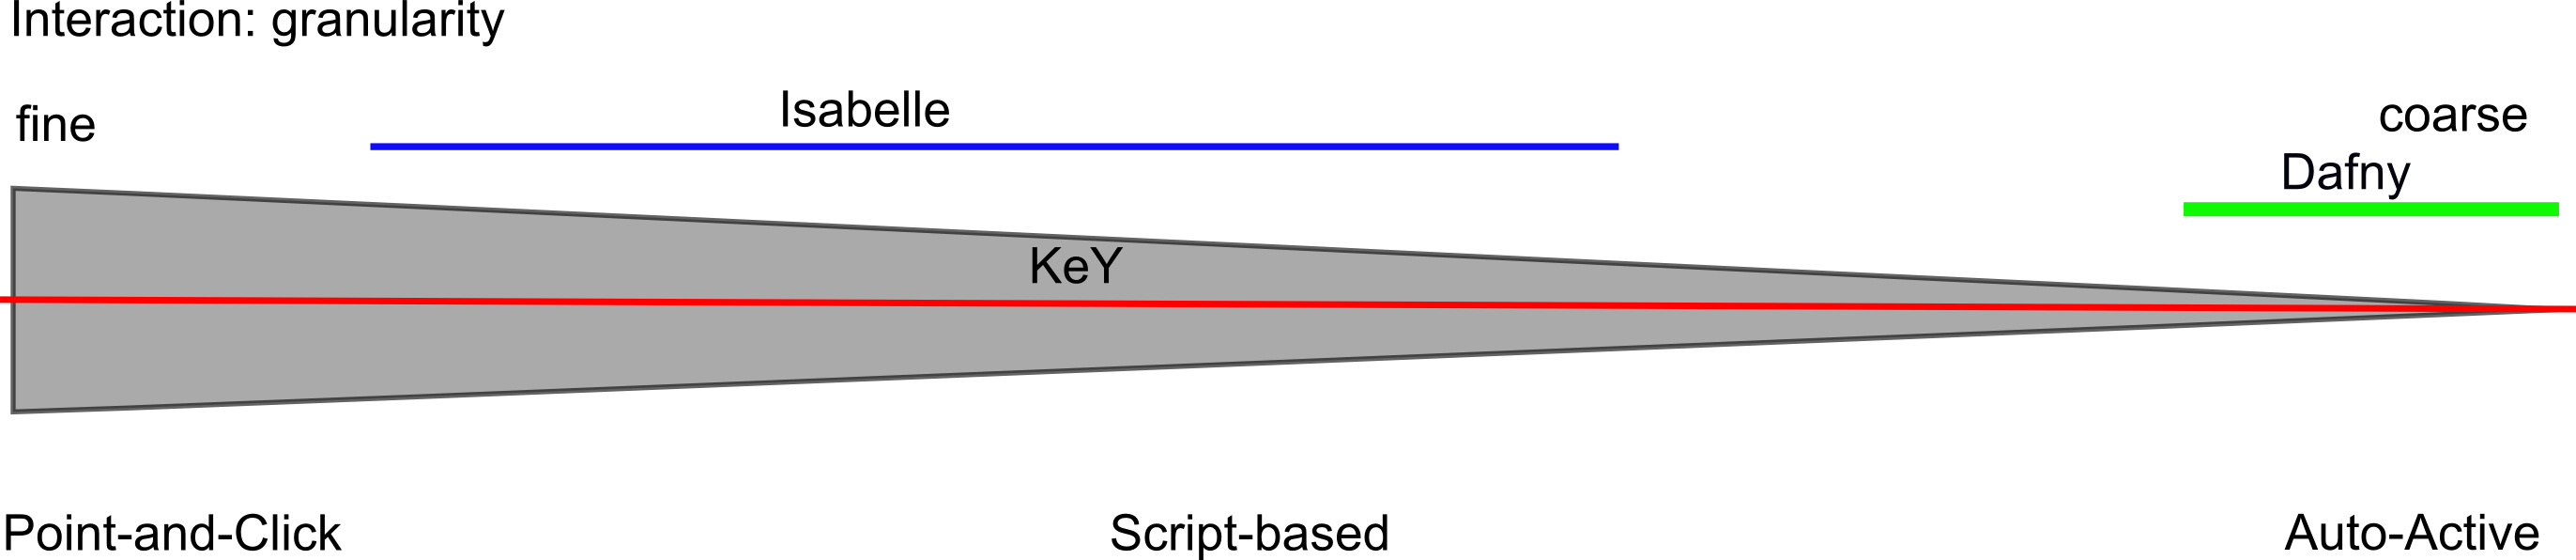
\includegraphics[width=1.1\textwidth]{../images/categorization.pdf}
% They differ in the granularity of interaction, level of interaction, type of 
% interaction, 
%  \item all principles have realized issues and added helpful additional 
% features (Z3 inspector, triggers, counter example 
% generator, abstraction mechanisms)
%  \item $\rightarrow$ however, there is no holistic approach allowing 
% interaction on the transition between autoactive and interactive verification

% \end{frame}
% \begin{frame}[c]{Interactive Point-and-Click}
% 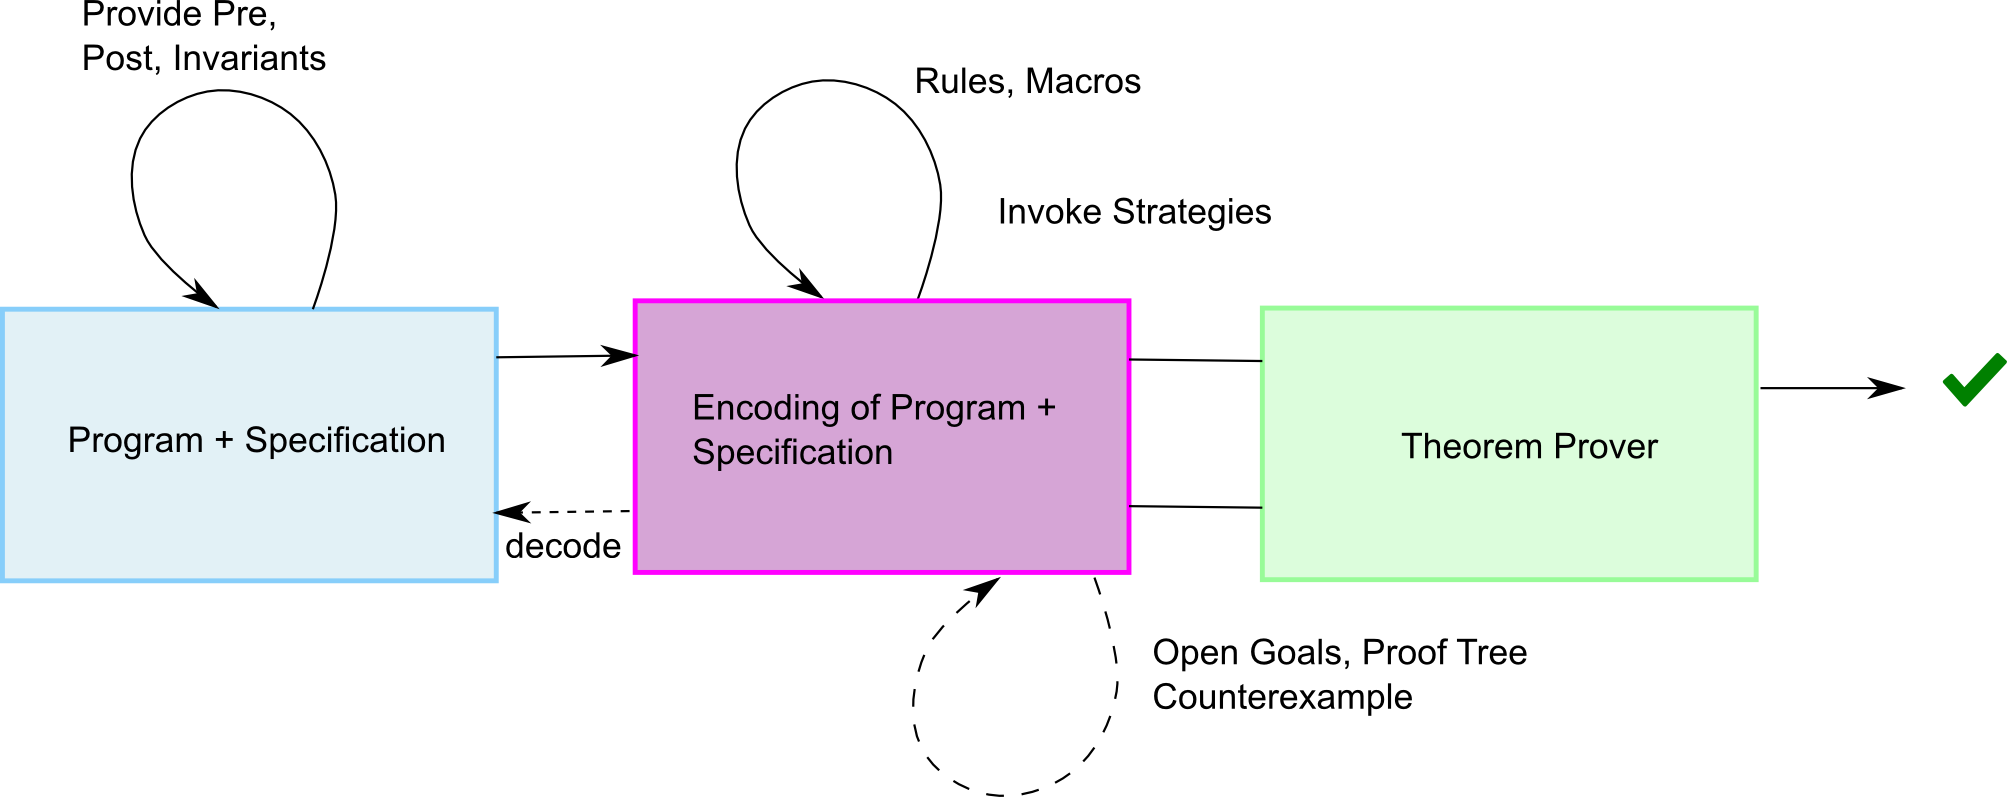
\includegraphics[width=\textwidth]{../images/interactive.pdf}
% \end{frame}
% 
% \begin{frame}[c]{Autoactive}
% 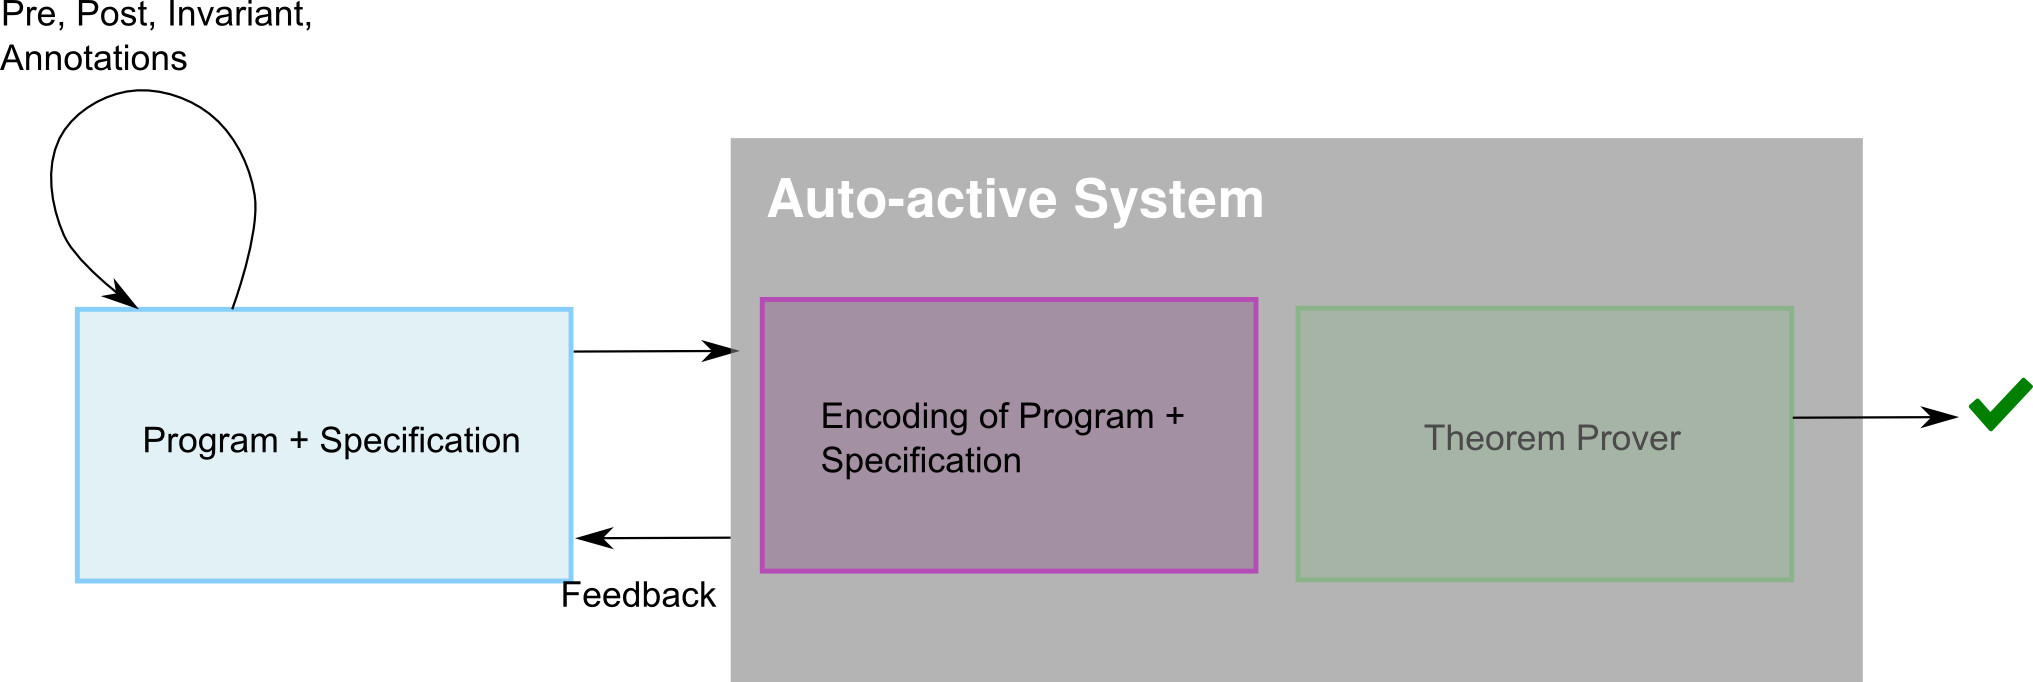
\includegraphics[width=1\textwidth]{../images/autoactive.pdf}
% \end{frame}
% 
% \begin{frame}[c]{Text/Script-Based Interaction}
% \hspace{6em}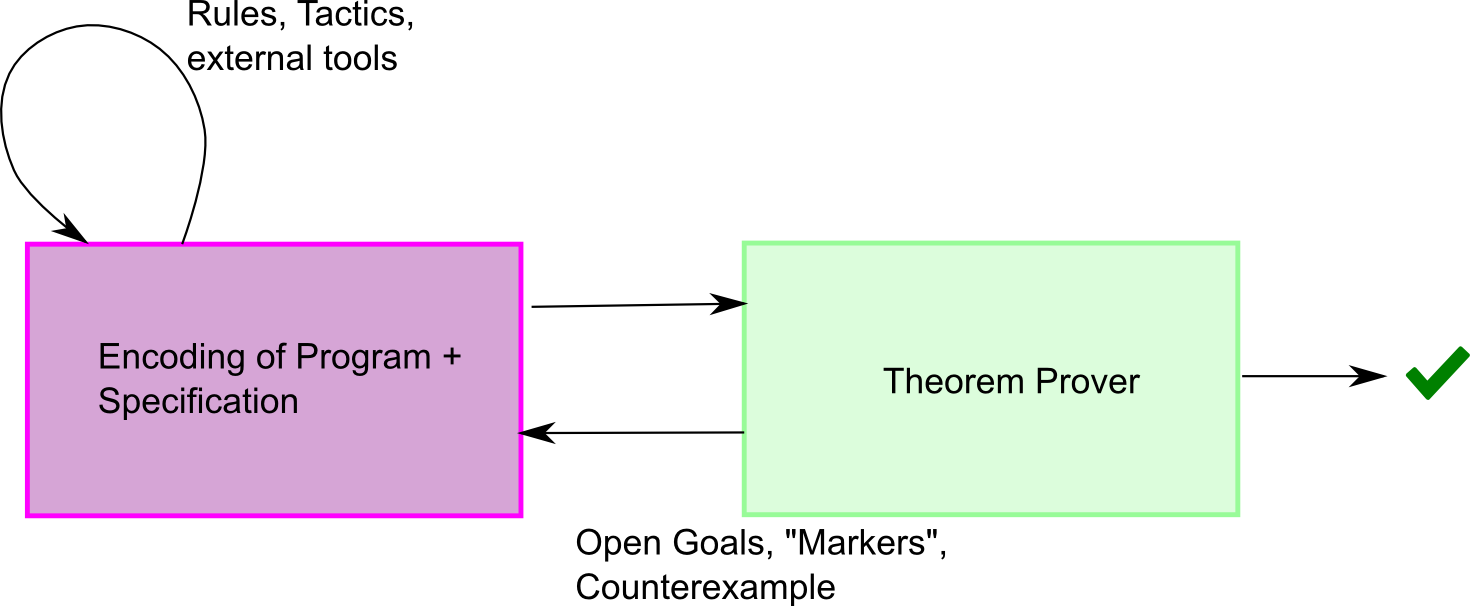
\includegraphics[width=.75\textwidth]{../images/tui.pdf}
% \end{frame}

% \begin{frame}[c]{Interactive Point-and-Click}
% % \begin{block}{Level of Interaction (proof guidance)} 
% %  Problem input on program level, proof guidance on logical level (two mental 
% % models)
% % \end{block}
% % % 
% % \begin{block}{Level of Feedback} 
% %  On logical level by showing the proof tree with open goals and sequent, macro 
% % (auto-pilot)
% % \end{block}
% % \begin{block}{User support during proof construction} 
% %  automatic heuristics, macros, counter examples, symbolic execution tree
% % \end{block}
% \begin{block}{Pros and Cons}
%  \begin{itemize}
%   \item[\textcolor{darkgreen}{\textbf{+}}/\textcolor{darkred}{\textbf{-}}] all 
% necessary information available
%   \item[\textcolor{darkgreen}{\textbf{+}}]full proof control
%   \item[\textcolor{darkred}{\textbf{-}}] interaction can be tedious
%   \item[\textcolor{darkred}{\textbf{-}}] error recovery 
%   \item[\textcolor{darkred}{\textbf{-}}] two mental models have to be kept in 
% sync
%  \end{itemize}
% 
% \end{block}
% \end{frame}
% 
% 
% 
% \begin{frame}[c]{Autoactive}
% 
% % \begin{block}{Level of Interaction (proof guidance)} 
% % Program level using annotations and programing constructs
% % \end{block}
% % % \vspace{2em}
% % \begin{block}{Level of Feedback} 
% % Program level using squiggly red lines, state 
% % inspection and counter example, path in program, hover text with useful 
% % information
% %  
% % \end{block}
% % \vspace{2em}
% % \begin{block}{User support during proof construction} 
% % inference of simple 
% % annotations, feedback on program level, useful hints in hover text of feedback, 
% % fast error recovery 
% % \end{block}
% \begin{block}{Pros and Cons}
%  \begin{itemize}
%   \item[\textcolor{darkgreen}{\textbf{+}}]interaction on input representation 
% $\rightarrow$ only one mental model
%   \item[\textcolor{darkgreen}{\textbf{+}}]comprehensible annotations
% \item[\textcolor{darkred}{\textbf{-}}] missing detailed insight into logical 
% level when proof attempt fails 
% \item[\textcolor{darkred}{\textbf{-}}] leaky abstraction
%  \end{itemize}
% 
% \end{block}
% 
% %  \begin{itemize}
% %   \item communication between prover and user on program level (one mental 
% % model)
% %   \item prover guidance through annotations
% %   \item no insight into logical level
% %   \item support in proof process: automatic proof search, inference of simple 
% % annotations
% %   \item support when proof attempt fails: counterexample (if it exists), 
% % verification debugger (view program states), \emph{intelligent} feedback using 
% % hovertext and squiggly red lines, direct manipulation and correction of program
% % 
% %  \end{itemize}
% 
% \end{frame}
% 
% 
% 
% %  \begin{itemize}
% %   \item interaction on logical level, problem formulation in terms of program 
% % (two mental models have to be kept in sync)
% % \item fine-grained interaction, many proof steps
% % \item full control of proof process
% % \item support in proof process: automatic heuristics, macros, SMT-solver support
% % \item support when proof attempt fails: counterexample, open goals (with large 
% % sequent) and large proof tree, some filter mechanisms for proof tree, search 
% % mechanisms, counter example generator
% % 
% %  \end{itemize}
% 
% % \end{frame}
% 
% \begin{frame}[c]{Text/Script-Based interaction}
% % \begin{block}{Level of Interaction (proof guidance)} 
% %  Problem input on program level, proof guidance on logical level (two mental 
% % models)
% % \end{block}
% % 
% % \begin{block}{Level of Feedback} 
% %  On logical level by showing open goals, Nitpick, Sledgehammer
% % \end{block}
% % \begin{block}{User support during proof construction} 
% %  tactics, counter examples, \emph{sorry} to postpone proof tasks and 
% % concentrate on one problem at a time
% % \end{block}
% \begin{block}{Pros and Cons}
%  \begin{itemize}
%   \item[\textcolor{darkgreen}{\textbf{+}}] problem/proof decomposition in 
% smaller parts
%   \item[\textcolor{darkgreen}{\textbf{+}}] interaction steps more coarse grained 
% than point-and-click 
% $\rightarrow$ more readable/comprehensible and proof plan expressible
%   \item[\textcolor{darkgreen}{\textbf{+}}/\textcolor{darkred}{\textbf{-}}] 
% limited insight into logical level
% \item[\textcolor{darkred}{\textbf{-}}] two mental models may have to be kept in 
% sync
%   
%  \end{itemize}
% 
% \end{block}
% 
% % \begin{itemize}
% %   \item interaction on textual level (console-like)
% %   \item dividing proof problem into subproblem and individually solve these
% %   \item still two mental models (proof script  and program)
% %   \item coarse-grained proof steps, comprehensible for human, proof plan 
% % expressible
% %   \item limited insight into logical level
% %   \item support for proof process: use lightweight tools at the beginning to 
% % solve easy problems, change of proof easy, simplification tactics for goals
% %   \item support when proof attempt fails: counterexample generator, 
% % sledgehammer to isolate problem, \emph{sorry} to postpone proof tasks
% % 
% %  \end{itemize}
% 
% \end{frame}
% 
% 
\begin{frame}{Seamless Integration}
Interaction concept supporting
\begin{itemize}
 \item interactive
 \item semi-automated
 \item seamless
\end{itemize}
proof guidance for an effective and efficient proof process. \\
\vspace{2em}
Support:
\begin{itemize}
 \item comprehension of failure of proof attempt
 \only<2->{ \begin{itemize}
  \item feedback on input language
  \item lightweight tools to discharge simple proof problems
  \item modularize proof
 \end{itemize}
}
 \item advancing proof
\only<3->{ \begin{itemize}
  \item proof exploration
  \item fast error recovery
 \end{itemize}
}
\end{itemize}

% 
% \begin{itemize}
%  \item Stay as long as possible input language of user is program
%  \item seamless integration of different existing methods 
%   \item allow for interaction on the transition between program and logical 
% level (show dependencies between different elements)
%  \item support user in finding orientation when proof attempt fails
%  \item support user in proof exploration
%   \item prototypically implement approach
%  \end{itemize}
% 
\end{frame}
% 
% 
\begin{frame}[t]{Decrease Costs of Iterations}
\begin{block}{Goal:}
\vspace{1ex}
 Interaction on suitable abstraction level \only<2->{(problem and user 
dependent)}
\end{block}
\vspace{2ex}

\only<3->{\begin{block}{Decrease number of level-changes}
\begin{itemize}
 \item stay on input language as long as possible (input and feedback)
 \item coarse proof steps (proof plan)
 \item clear overview over overall proof state
\end{itemize}
 
\end{block}
}
\vspace{2ex}

\only<4->{\begin{block}{Decrease cost per level-change}

 \begin{itemize}
  \item state inspection on logical level
  \item visible dependencies between levels
  \item proof exploration on logical level
 \end{itemize}

\end{block}
}


% \begin{itemize}
%  \item Stay on input language as long as possible (input and feedback)
%  \item Allow for coarse proof steps (proof plan)
%  \item Give clear overview over overall proof state
%  \item If necessary allow for state inspection on logical level
%  \item Ease transition between program and logic by making dependencies visible
%  \item Allow for fast error recovery
%  \item Allow for proof exploration on logical level
% \end{itemize}
% 
 
\end{frame}

\begin{frame}{Artifact Hierarchy in Interactive Verifications Process}
 TODO Bild
\end{frame}

% 
% \begin{frame}[t]{Architecture}
%  \begin{figure}
%   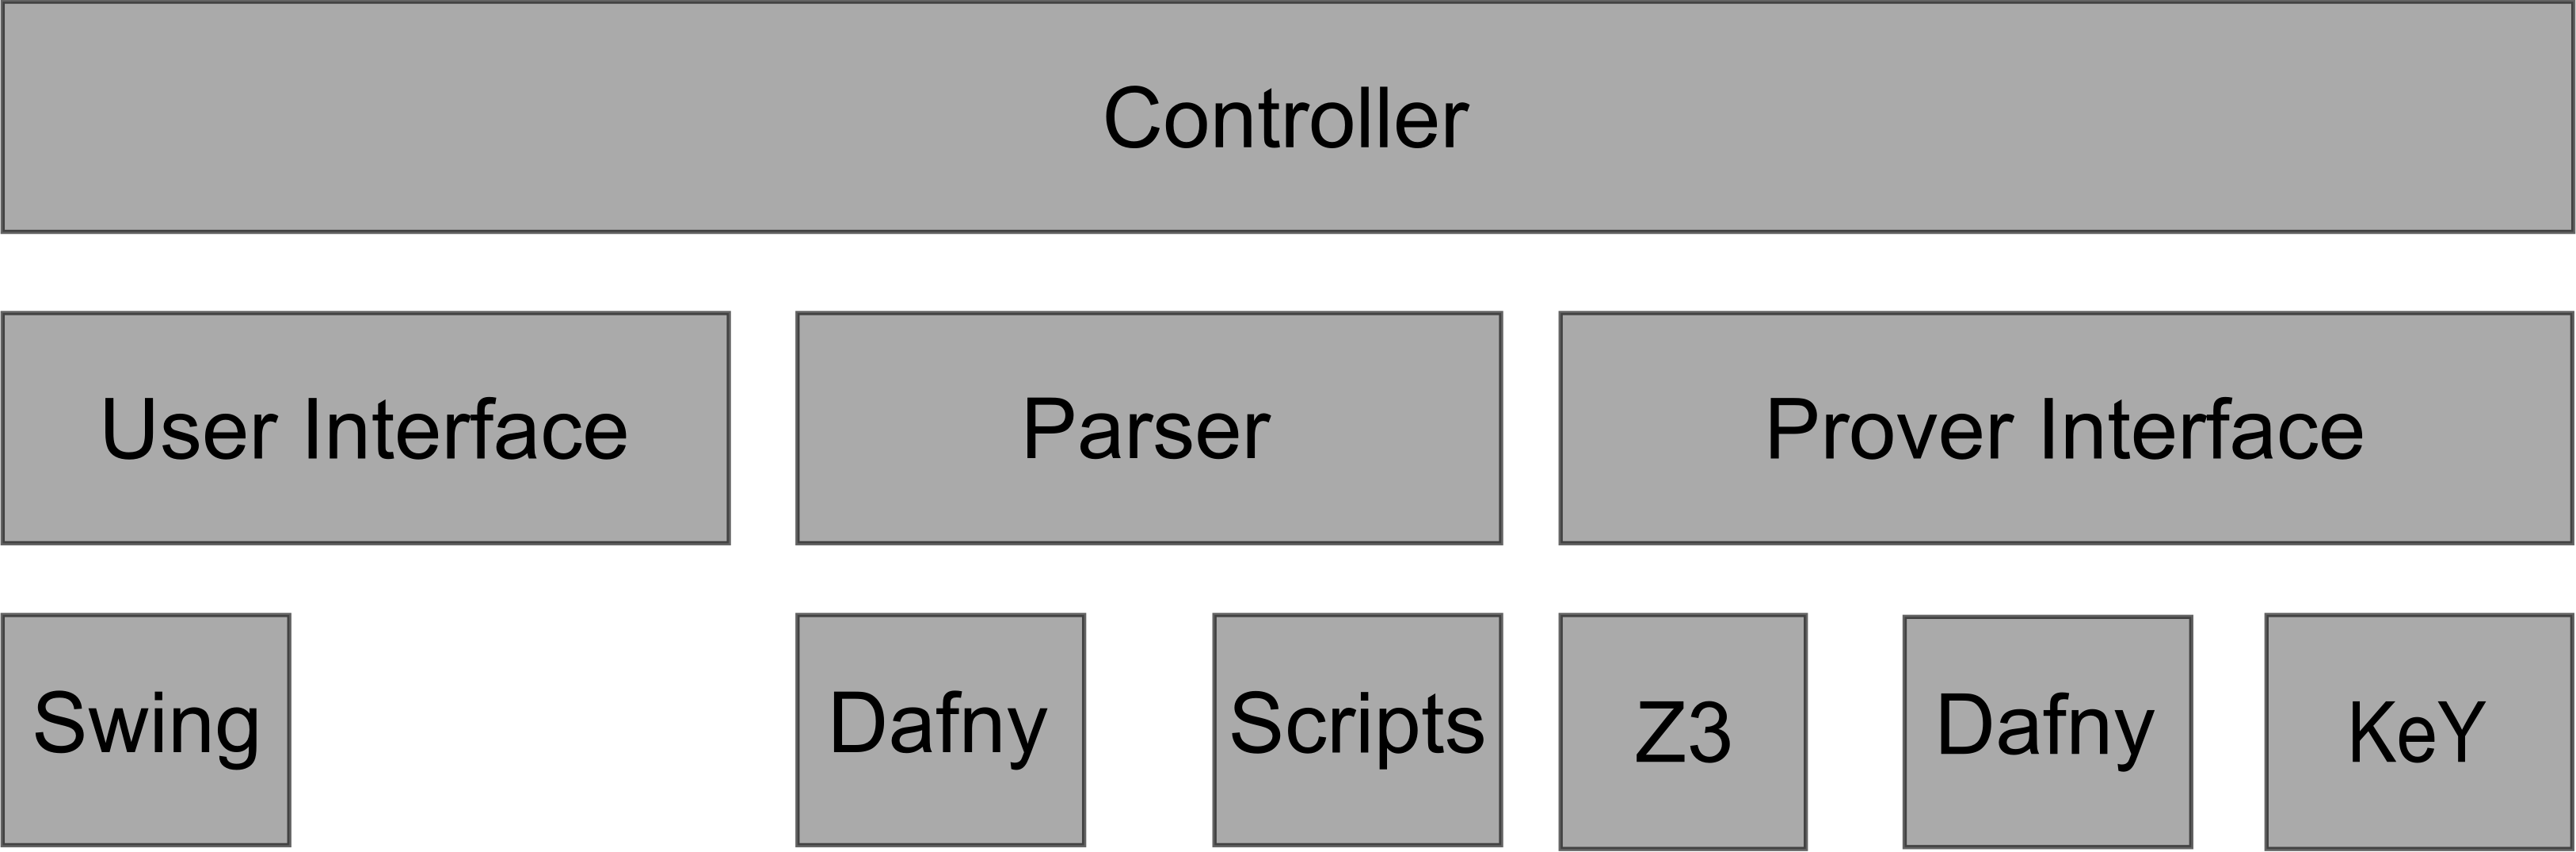
\includegraphics[width=.9\textwidth]{../images/aufbau.pdf}
%  \end{figure}
% 
% \end{frame}
% 
% 
% \begin{frame}[t]{Architecture}
%  \begin{figure}
%   \includegraphics[width=.9\textwidth]{../images/aufbau1.pdf}
%  \end{figure}
% 
% \end{frame}
% 
% 
% 
% \begin{frame}[t]{Example}
%  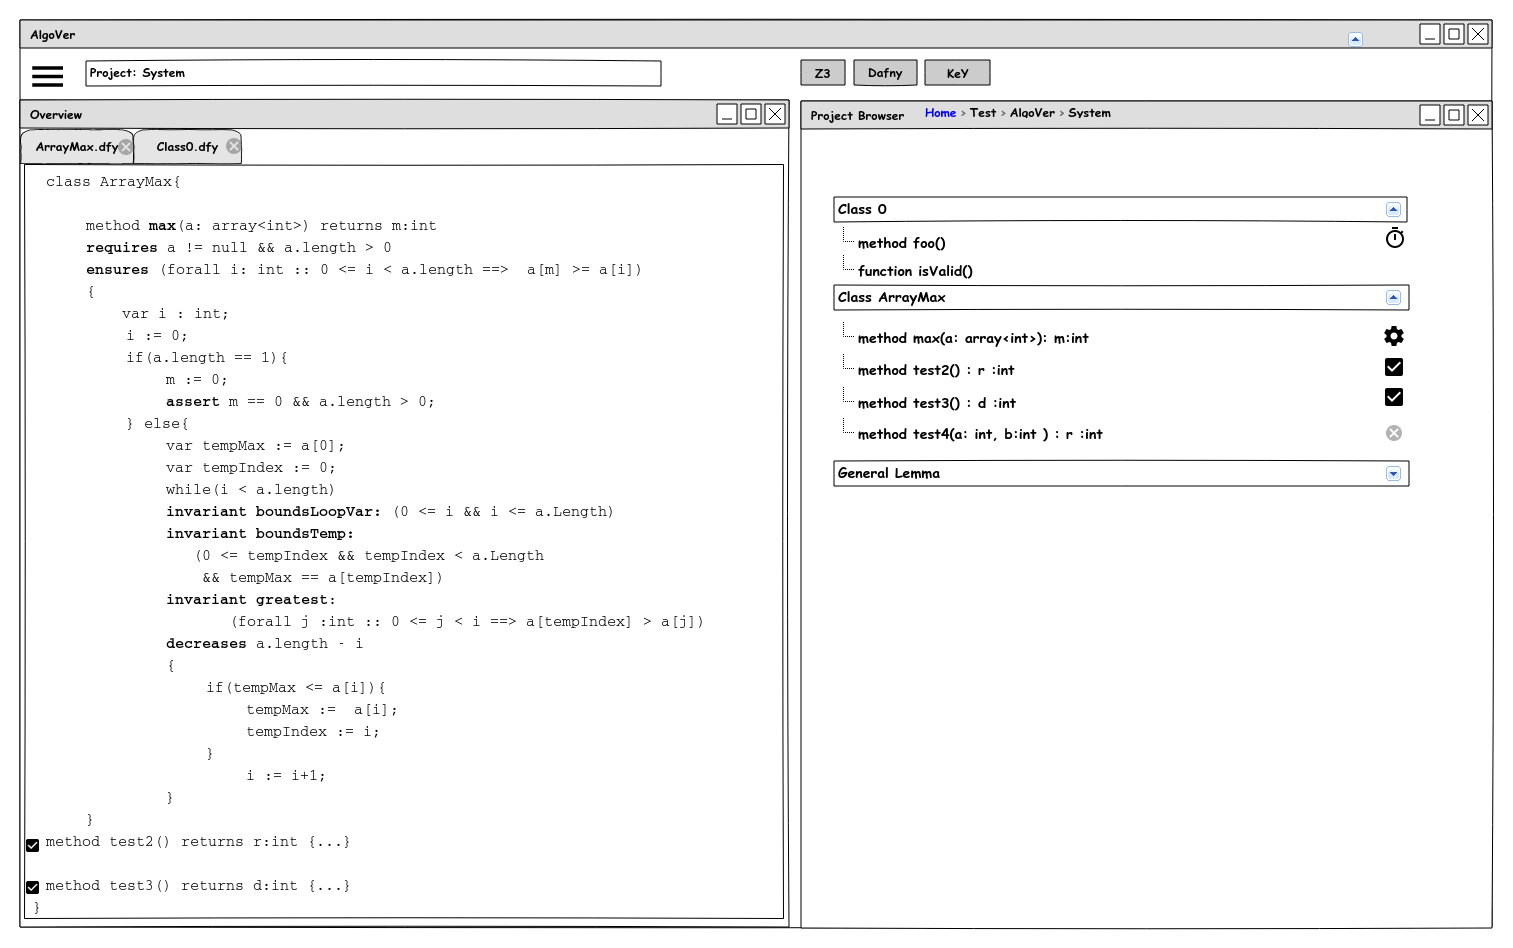
\includegraphics[width=\textwidth]{../../mockups/pics/afterloading2.png}
% \end{frame}
% 
% \begin{frame}[t]{Example}
%  \includegraphics[width=\textwidth]{../../mockups/pics/afterloading2a.png}
% \end{frame}
% 
% 
% \begin{frame}[t]{Example}
%  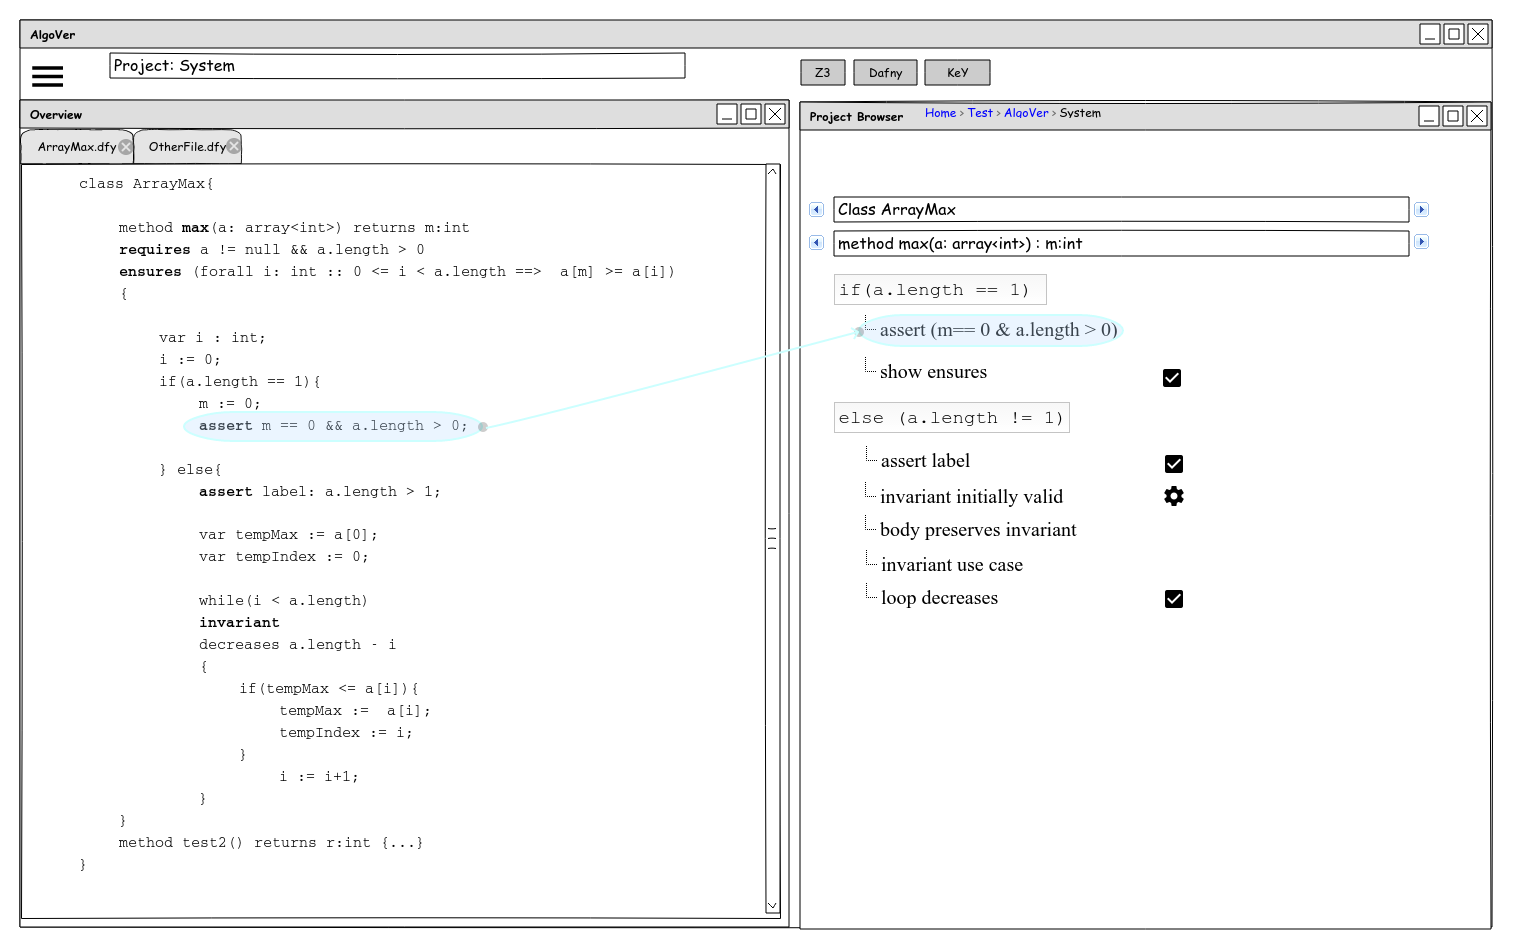
\includegraphics[width=\textwidth]{../../mockups/pics/moreconcreteview.png}
% \end{frame}
% 
% \begin{frame}[t]{Example}
%  \includegraphics[width=\textwidth]{../../mockups/pics/moreconcreteviewa.png}
% \end{frame}
% 
% \begin{frame}[t]{Example}
%  \includegraphics[width=\textwidth]{../../mockups/pics/moreconcreteviewb.png}
% \end{frame}
% 
% 
% \begin{frame}[t]{Example}
%  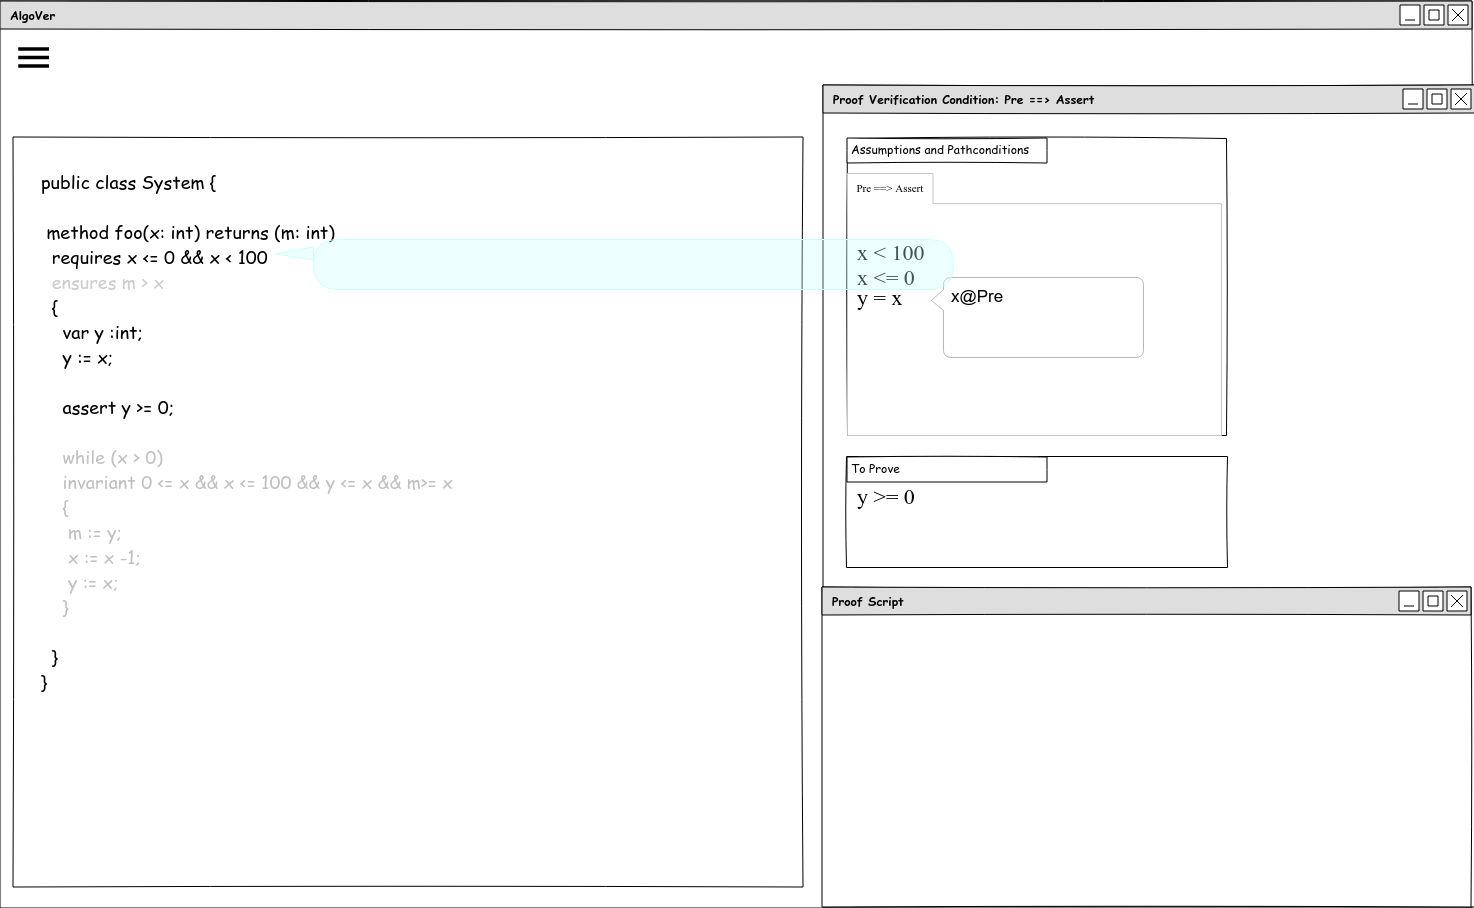
\includegraphics[width=\textwidth]{../../mockups/pics/pvc_log_view.png}
% \end{frame}
% 
% \begin{frame}[t]{Example}
%  \includegraphics[width=\textwidth]{../../mockups/pics/pvc_log_viewa.png}
% \end{frame}
% 
% 
% \begin{frame}[t]{Example}
%  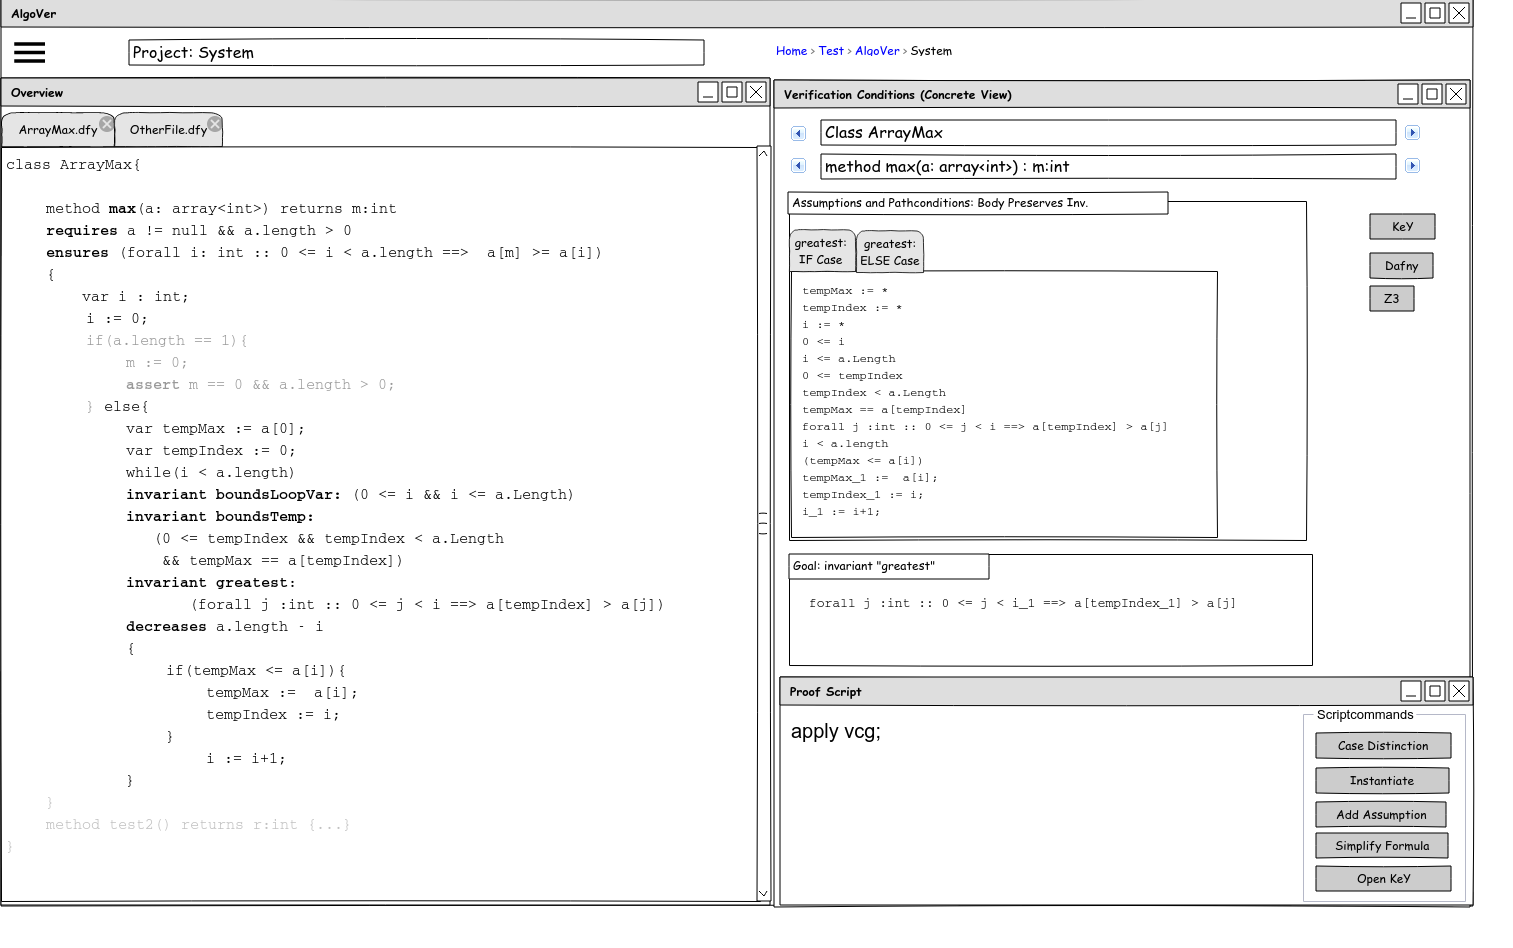
\includegraphics[width=\textwidth]{../../mockups/pics/pvcdetailview.png}
% \end{frame}
% 
% \begin{frame}[t]{Example}
%  \includegraphics[width=\textwidth]{../../mockups/pics/pvcdetailviewa.png}
% \end{frame}
% 
% 
% \begin{frame}[t]{Example}
%  \includegraphics[width=\textwidth]{../../mockups/pics/pvcdetailview_2.png}
% \end{frame}
% 
% \begin{frame}[t]{Example}
%  \includegraphics[width=\textwidth]{../../mockups/pics/pvcdetailview_2a.png}
% \end{frame}
% 
% 
% \begin{frame}[t]{Example}
%  \includegraphics[width=\textwidth]{../../mockups/pics/pvcdetailview_3.png}
% \end{frame}
% 
% \begin{frame}[t]{Example}
%  \includegraphics[width=\textwidth]{../../mockups/pics/pvcdetailview_3a.png}
% \end{frame}
% 
% 
% \begin{frame}[t]{Example}
%  \includegraphics[width=\textwidth]{../../mockups/pics/pvcdetailview_4.png}
% \end{frame}
% 
% \begin{frame}[t]{Example}
%  \includegraphics[width=\textwidth]{../../mockups/pics/pvcdetailview_4a.png}
% \end{frame}


\begin{frame}[c]{Summary}
Bridging interaction gap between code and logic by
 \begin{itemize}
  \item fluent transition between levels
  \item different coupled proof views
  \item interaction on all levels
  \item seamless integration of sophisticated methods
 \end{itemize}
\begin{block}{Future Work}
 \begin{itemize}
  \item implement concept 
  \item evaluate concept with users
 \end{itemize}

\end{block}

\end{frame}

% \begin{frame}[c]{Discussion}
% \centering{In your experience:}\\
% \bigskip
% \centering{What is the bottleneck for interaction?}
% 
% 
% \end{frame}

% 
% \begin{frame}{Requirements}
% \begin{itemize}
%  \item interaction on Input language as long as possible
%  
%  \item verification conditions
%  \item use lightweight tools to solve simple/easy verification conditions
%  \item small counterexamples
%  \item proof process iterative $\rightarrow$ fast feedback
%  \item dependencies always visible to user on demand
%  \item support for proof exploration (what if...)
% %  \item support when proof attempt fails: pvc mapping back to source code (with 
% % greying out), possibility to change to logical level with support of 
% % dependencies, 
% %  
% \end{itemize}
% 
%  
% \end{frame}
% 
% \begin{frame}{Concept}
%  \begin{itemize}
%   \item allow user to view projections of the proof state in different 
% domains (program domain, logical domain, abstract logical domain) and interact 
% on all domains
%  \item support user in stepwise changing views
%  \item support of exploration process during proof construction
%  \item use existing tools as underlying methods
%   
%  \end{itemize}
% 
% \end{frame}

\end{document}
 
